\documentclass[letterpaper, 11pt, colorful, sections]{jiahua}
\title{Math 1010: Analysis \textit{Lecture Notes}}
\author{J. Serrano}
\date{Spring 2023}

\usepackage[textsize=tiny, textwidth=18mm]{todonotes}
\setuptodonotes{noline, color=green!20}
\usepackage{cancel}
\usetikzlibrary{cd}
\numberwithin{equation}{section}

\usepackage[all,cmtip]{xy}

\begin{document}
\maketitle
\begin{quote}
    \quad These are lecture notes for ``Math 1010: Analysis: Functions of One Variable'' taught at \textsc{Brown University} by Javi G\'omez Serrano in the Spring of 2023.

    \quad These notes are taken by Jiahua Chen with gracious help and input from classmates. Please direct any mistakes/errata to me via \href{mailto:jiahua_chen2@brown.edu}{email}, or feel free to pull request the notes repository (\url{https://github.com/jchen/math1010-notes}).

    \quad Notes last updated \today.
\end{quote}
\tableofcontents
\bibliographystyle{alpha}
\bibliography{bibliography}

\newpage
%!TEX root = ../notes.tex
\section{January 26, 2023}
\subsection{Introductions}
\textbf{Instructor:} Javi G\'omez Serrano. Email: \href{mailto:javier_gomez_serrano@brown.edu}{javier\_gomez\_serrano@brown.edu}.

\textbf{Text:} \emph{Principles of Mathematical Analysis}\footnote{Find online using \emph{appropriate channels}.}, W. Rudin \cite{rudin1976principles}. We will cover select chapters of this book. If the pace is too fast, bring it up.

\textbf{Structure:} Biweekly HW with problems from the book and extra problems. Homework posted Thursdays. Roughly 6 homework assignments (maybe 5, or 7). Worst homework will be dropped.

Midterm and final, in class (TBA). There will additionally be 2 quizzes (20 minutes each), which should be extremely easy. There are 2 questions from the quizzes: one will literally be a problem from the homework, and one will be a definition.

Grading potentially returned by Tuesday following submission. Grading is as follows: 30\% problem sets, 10\% quizzes, 25\% midterm, 35\% final. There will be a curve.

\textbf{Office Hours:} Kassar 314, Monday 5-7pm.

\subsection{Fundamentals}
\subsubsection{Sets}
\begin{definition}[Set]
    One can think of a \ul{set} as a collection of objects.

    If $a$ is an object, and $A$ is a set. $a\in A$ means that $a$ is a \ul{member} of $A$.
\end{definition}
\begin{definition}[Subsets]
    If $A, B$ are sets, we say that $A$ is a \ul{subset} of $B$ (we write $A\subset B$\framedfootnote{Some also write $A\subseteq B$.}) whenever $a\in A\implies a\in B$.

    $A$ is a \ul{proper} subset of $B$ if $A\subset B$ and $A\neq B$.
\end{definition}
\begin{remark}
    $\emptyset$ is the set with no elements. $\emptyset$ is a subset of \emph{every} set.
\end{remark}
\begin{definition}[Union]
    If $A, B$ are sets, $A\cup B$ is the \ul{union} of $A$ and $B$.
    \[A\cup B \overset{\text{def}}{=}\left\{ a\mid a\in A \text{ or }a\in B \right\}\]
\end{definition}
\begin{definition}[Intersection]
    If $A, B$ are sets, $A\cap B$ is the \ul{intersection} of $A$ and $B$.
    \[A\cap B \overset{\text{def}}{=}\left\{ a\mid a\in A \text{ and }a\in B \right\}\]
\end{definition}
We can generalize this to an arbitrary number of sets:
\begin{definition}[Generalization of Union/Intersection]
    If $\mathcal{C}$ is a collection of sets (possibly infinite). Then
    \[\bigcup_{A\in \mathcal{C}}A \overset{\text{def}}{=} \{a\mid a\in A \text{ for some }a\in \mathcal{C}\}\]
    and
    \[\bigcap_{A\in \mathcal{C}}A \overset{\text{def}}{=} \{a\mid a\in A \text{ for all }A\in \mathcal{C}\}.\]
\end{definition}
\begin{definition}[Disjunction]
    We say that $A$ and $B$ are \ul{disjoint} if $A\cap B = \emptyset$.
\end{definition}
\begin{proposition}[Distribution over intersection and union]
    The following is true:
    \begin{enumerate}
        \item $A\cap(B\cup C) = (A\cap B) \cup (A\cap C)$
        \item $A\cup(B\cap C) = (A\cup B) \cap (A\cup C)$
    \end{enumerate}
\end{proposition}
\begin{proof}[Proof of statement 1.]
    We prove that the sets on the left are contained in the sets on the right, and the sets on the right are contained on the sets on the left. That is, $X\subset Y$ and $Y\subset X$ $\Rightarrow$ $X = Y$.

    \begin{description}
        \item[Case $A\cap(B\cup C)\subset(A\cap B) \cup (A\cap C)$:] Let $a\in A\cap (B\cup C)$. Then $a\in A$ and $a\in (B\cup C)$. So $a\in B$ or $a\in C$.

            Suppose $a\in B$, then $a\in A\cap B$ so $a\in (A\cap B)\cup (A\cap C)$. Suppose $a\in C$, then $a\in A\cap B$ so still $a\in (A\cap B)\cup (A\cap C)$.

            Regardless, this is precisely the set on the right.
        \item[Case $(A\cap B) \cup (A\cap C)\subset A\cap(B\cup C)$:] Let $a\in (A\cap B) \cup (A\cap C)$. Then $a\in (A\cap B)$ or $a\in (A\cap C)$.

            If $a\in (A\cap B)$, then $a\in A$ and $a\in B$, so $a\in A$ and $a\in B\cup C$, so $a\in A\cap(B\cup C)$.

            If $a\in (A\cap C)$, then $a\in A$ and $a\in C$, so $a\in A$ and $a\in B\cup C$, so still $a\in A\cap (B\cup C)$.

            Again, regardless, $a\in A\cap (B\cup C)$.
    \end{description}
    Having proven containment in both directions, we conclude the sets on the left and right are equal.
\end{proof}

\begin{definition}[Set Difference]
    We define the \ul{difference} $A\setminus B$ as
    \[A\setminus B = \{a\mid a\in A, a\not\in B\}.\]
    \begin{center}
        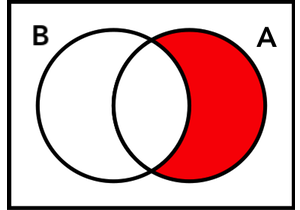
\includegraphics[width=0.3\textwidth]{images/set_difference.png}
    \end{center}
\end{definition}
\begin{definition}[Symmetric Difference]
    We define the \ul{symmetric difference}
    \[A\triangle B = (A\setminus B)\cup (B\setminus A).\]
    \begin{center}
        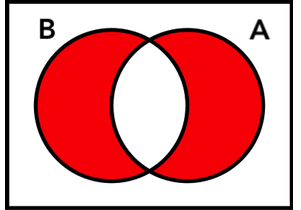
\includegraphics[width=0.3\textwidth]{images/set_sym_difference.png}
    \end{center}
\end{definition}
\begin{definition}[Set Product]
    We define the \ul{product} of $A$ and $B$ as
    \[A\times B = \{(a, b)\mid a\in A, b\in B\}\]
\end{definition}

\subsubsection{Relations}
\begin{definition}[Relations]
    A \ul{relation} $R$ between sets $A$ and $B$ is any subset of $A\times B$.

    If $(a, b)\in R$, we will think of $a$ ``being related'' to $b$.
\end{definition}

For now, consider $A = B$. We define a special set of relations.
\begin{definition}[Reflexive/Symmetric/Transitive Relations]\label{defn:rst-relations}
    We have the following definitions:
    \begin{enumerate}
        \item $R$ is \ul{reflexive} iff $(a, a)\in R, \forall a\in A$.\framedfootnote{$\forall$ is to say `for all'.}
        \item $R$ is \ul{symmetric} iff whenever $(a_1, a_2)\in R$, then $(a_2, a_1)\in R$.
        \item $R$ is \ul{transitive} iff whenever $(a_1, a_2)\in R$, and $(a_2, a_3)\in R$, then $(a_1, a_3)\in R$.
    \end{enumerate}
\end{definition}

\begin{definition}[Equivalence Relation]
    A relation $R$ that satisfies all conditions 1-3 in \cref{defn:rst-relations} is called an \ul{equivalence relation}.
\end{definition}

\begin{definition}[Equivalence Class]
    Given an element $a\in A$ with relation $R$, we write
    \[[a]_R \overset{\text{def}}{=} \{a' \in A\mid (a, a')\in R\}\]
    as the \ul{equivalence class} of $a$ (the set of all elements that are `related' to $a$).
\end{definition}
\begin{remark}
    Instead of writing $(a, a')\in R$, we write $a\sim_R a'$ or $a\sim a'$.
\end{remark}

\begin{proposition}[Distinct Equivalence Classes are Disjoint]
    If $R$ be an equivalence relation on $A$. Suppose $a_1, a_2\in A$. Then, either
    \[[a_1]_R = [a_2]_R\quad \text{or}\quad [a_1]_R\cap [a_2]_R = \emptyset\]
\end{proposition}
\begin{proof}
    We show that these statements cannot happen simultaneously, and that one or the other \emph{must} be true.

    The former is as follows: notice $a_1\in [a_1]_R$ because $a_1\sim a_1$ by $R$ reflexive. Since $[a_1]_R = [a_2]_R$, then $a_1\in [a_1]_R\cap [a_2]_R$. This implies that the intersection $[a_1]_R\cap [a_2]_R$ is nonempty, which is a contradiction.

    We now show that at least one has to happen. If $a_1\in [a_1]_R\cap [a_2]_R = \emptyset$, we are done. Otherwise, if $a_1\in [a_1]_R\cap [a_2]_R \neq \emptyset$, then $\exists\footnote{$\exists$ is to denote `there exists'.}a\in A$ such that $a\in[a_1]_R$ and $a\in[a_2]_R$.

    We claim \textsc{wlog} $[a]_R = [a_1]_R$. Suppose $a'\in [a]_R$, then $(a, a')\in R$. Since $(a,a')\in R$ and $(a_1, a)\in R$ (due to $a\in [a_1]_R$), transitivity gives $(a_1, a')\in R$ so $a'\in[a_1]_R$. Let's otherwise suppose $a'\in [a_1]_R$, so $(a_1, a')\in R$. Reflexivity gives $(a, a_1)\in R$ ($(a_1, a)\in R$ by $a\in [a_1]_R$), and by transitivity $(a,a_1)\in R$ and $(a_1, a')\in R$ gives $(a, a')\in R$ so $a'\in [a]_R$.\footnote{Wow, this is quite dense but the idea is to chain reflexivity and transitivity to get everything related to one another.}

    By symmetry, $[a]_R = [a_2]_R$, so $[a_1]_R = [a]_R = [a_2]_R$ which is as desired.
\end{proof}

Essentially, what we have shown, is that we can partition a set according to equivalence classes. All equivalence classes are either going to be the same or different. This is, equivalence relations form a \emph{partition} of a set. We can construct a set of partitions (disjoint subsets) of a set $S$. That is, ``equivalence classes partition $A$.''

\begin{definition}[Partition]
    A \ul{partition} of $A$ is a collection $\mathcal{P}$ of subsets of $A$ such that
    \begin{enumerate}
        \item $A = \bigcap_{S\in \mathcal{P}}S$,
        \item $S_i\cap S_j = \emptyset$ if $S_i\neq S_j$ for each $S_i, S_j\in \mathcal{P}$.
    \end{enumerate}
\end{definition}

With this definition, if $R$ is an equivalence relation, then $\mathcal{C}_R = \{[a]_R\mid a\in A\}$ is a partition of $A$.

We'll use all of this to define a function (which is the whole purpose of this course).

\subsubsection{Functions}
\begin{definition}[Function]
    Let $A, B$ be sets and $f$ be a relation between $A$ and $B$.

    We say $f$ is a \ul{function} from $A$ to $B$ and we write $f: A\to B$ iff the following holds:
    \begin{enumerate}
        \item $\forall a\in A$, there exists \emph{at least} one $b\in B$ s.t. $(a, b)\in f$. (all elements have an image)
        \item $\forall a\in A$, there exists \emph{at most} one $b\in B$ s.t. $(a, b)\in f$. (all elements have only one image)
    \end{enumerate}
    We write $f(a) = b$, and $b$ is the \ul{image} of $a$ by $f$. We call $A$ the domain of $f$, and $B$ the codomain of $f$\framedfootnote{I like to denote $B$ the codomain and the actual set of images the \emph{image} of $f$. And `range' is just ambiguous it seems.}.
\end{definition}
%!TEX root = ../notes.tex
\section{January 31, 2023}

\subsection{Properties of Functions}
\begin{definition}[Injectivity]
    A function $f: A\to B$ is \ul{injective} (one-to-one) if
    \[f(a_1) = f(a_2)\implies a_1 = a_2.\]
    ``No two elements in $A$ map to the same element in $B$.''
\end{definition}

\begin{definition}[Surjectivity]
    A function $f: A\to B$ is \ul{surjective} (onto) if
    \[\forall b\in B, \exists a\in A, \text{ s.t. }f(a) = b.\]
    ``Every element in $B$ has a preimage in $A$.''
    % \todo{Diagram}
\end{definition}

\begin{definition}[Functional Composition]
    Suppose $f: A\to B$ and $g: B\to C$ are functions, then $(g\circ f): A\to C$ with
    \[(g\circ f)(a) := g(f(a))\]
    % \todo{Diagram}
\end{definition}

\begin{proposition}
    Let $f: A\to B$, $g: B\to C$ be functions, then if $f, g$ are both injective, then so is $(g\circ f)$.

    The same holds if they are surjective.
\end{proposition}
\begin{proof}[Proof of injective part]
    Let $a, a'\in A$ be such that
    \begin{align*}
        (g\circ f)(a) & = (g\circ f)(a') \\
        g(f(a))       & = g(f(a'))       \\
        \intertext{With $g$ injective, therefore}
        f(a)          & = f(a')
        \intertext{With $f$ injective, we then have}
        a             & = a'
    \end{align*}
    Therefore, $(g\circ f)$ is injective.
\end{proof}

\begin{proof}[Proof of surjective part]
    We want to show that $\forall c\in C$, $\exists a\in A$ such that $g(f(a)) = (g\circ f)(a) = c$.

    Since $g$ is surjective, $\exists b\in B$ s.t. $g(b) = c$.

    Since $f$ is surjective, $\exists a\in A$ such that $f(a) = b$.

    Now, plugging in, $g(f(a)) = g(b) = c$. Therefore, exists such a pre-image $a\in A$ for every $c\in C$ under $(g\circ f)$. Hence, $(g\circ f)$ is surjective.
\end{proof}

\begin{definition}[Bijectivity]
    If $f: A\to B$ is injective and surjective, we call $f$ a \ul{bijection}.
\end{definition}

\begin{theorem}[Existence of Inverse]
    Let $f: A\to B$, then $\exists f^{-1}: B\to A$ such that
    \begin{align*}
        f^{-1}\circ f = \mathrm{id}_A \\
        f\circ f^{-1} = \mathrm{id}_B
    \end{align*}
    where
    \begin{align*}
        \Id_A: A\to A, \quad \forall a\in A, \Id_A(a) = a \\
        \Id_B: B\to B, \quad \forall b\in B, \Id_B(b) = b
    \end{align*}
    if and only if $f$ is a bijection.
\end{theorem}
\begin{proof}
    ~\begin{description}
        \item[$\Longleftarrow$:] Suppose $f: A\to B$ is a bijection. Then, we define $f^{-1}\subset B\times A$ as
            \[f^{-1} = \{(b, a)\mid (a, b)\in f\}\]
            It's clear that this is a relation. We check that $f^{-1}$ is a function.

            That is, we need to check that $\forall b\in B$, there exists one and only one $a\in A$ such that $(b, a)\in f^{-1}$.

            In other words, taking the definition of $f^{-1}$, we have to check that $\forall b\in B$, $\exists!\footnote{$\exists!$ as `exists exactly one'.} a\in A$ such that $(a, b)\in f$. This is exactly $f$ being bijective.

            Let's now show that
            \begin{align}
                f^{-1}\circ f & = \Id_A \label{eq:inverse-1} \\
                f\circ f^{-1} & = \Id_B \label{eq:inverse-2}
            \end{align}

            Let's first show \cref{eq:inverse-1}, suffices to show $f^{-1}(f(a))\overset{?}{=}a, \forall a$.

            $\forall a\in A$, $\exists b\in B$ such that $f(a) = b$, so $(a, b)\in f$. By definition, $(b, a)\in f^{-1}$ so $f^{-1}(b) = a$. Then $f^{-1}(f(a)) = f^{-1}(b) = a$.

            We do \cref{eq:inverse-2} very similarly.

        \item[$\Longrightarrow$:] Suppose $f: A\to B$ and $g\footnote{We use $g$ to reduce confusion with $f^{-1}$}: B\to A$ such that $g\circ f = \Id_A$ and $f\circ g= \Id_B$. We show that $f$ is a bijection.

            We first show injectivity. Suppose $f(a_1) = f(a_2)$, applying $g$ on both sides gives
            \begin{align*}
                g(f(a_1))  & = g(f(a_2))  \\
                \Id_A(a_1) & = \Id_A(a_2) \\
                a_1        & = a_2
            \end{align*}
            This gives us injectivity.

            We then show surjectivity. Let $b\in B$, we claim $\exists a\in A$ such that $f(a) = b$. Take $a := g(b)$, then $f(a) = f(g(b)) = b$. We've found such an $a$ such that $f(a) = b$, giving us surjectivity.
    \end{description}
    In both directions, this gives us the bijection.
\end{proof}

\begin{remark}
    Let $f: A\to B$ be a bijection, with $A$ and $B$ finite. We have that $A$ has $n$ elements $\iff$ $B$ has $n$ elements. That is, $A$ and $B$ have equal cardinality.

    This extends to arguments on infinite sets too, like between $\ZZ$ and $\QQ$. $\QQ$ and $\RR$ or $\ZZ$ and $\RR$ have different cardinalities and hence don't have bijections.
\end{remark}

If $f: A\to B$ is not a bijection, we cannot define an inverse in the same way as we did before. But, we can consider the inverse image.

\begin{definition}[Inverse Image]
    Given function $f: A\to B$, $C\subseteq B$ we define the \ul{inverse image} of $C$ as
    \[f^{-1}(C) := \left\{ a\in A\mid f(a)\in C \right\}\]
    ``The set of $a\in A$ that take me somewhere in $C$.''
\end{definition}

If $C = \{b\}$, we get all elements mapped to $b$. That is,
\[f^{-1}(\{b\}) = \left\{ a\in A\mid f(a) = b \right\}\]

\subsection{Cardinality}


\end{document}